%
% File acl2014.tex
%
% Contact: giovanni.colavizza@epfl.ch
%%
%% Based on the style files for ACL-2013, which were, in turn,
%% Based on the style files for ACL-2012, which were, in turn,
%% based on the style files for ACL-2011, which were, in turn, 
%% based on the style files for ACL-2010, which were, in turn, 
%% based on the style files for ACL-IJCNLP-2009, which were, in turn,
%% based on the style files for EACL-2009 and IJCNLP-2008...

%% Based on the style files for EACL 2006 by 
%%e.agirre@ehu.es or Sergi.Balari@uab.es
%% and that of ACL 08 by Joakim Nivre and Noah Smith

\documentclass[11pt]{article}
\usepackage{acl2014}
\usepackage{times}
\usepackage{url}
\usepackage{latexsym}
\usepackage{graphicx}	% For figure environment
\usepackage{hyperref}
\usepackage{mathtools}

\DeclarePairedDelimiter\floor{\lfloor}{\rfloor}

%\setlength\titlebox{5cm}

% You can expand the titlebox if you need extra space
% to show all the authors. Please do not make the titlebox
% smaller than 5cm (the original size); we will check this
% in the camera-ready version and ask you to change it back.


\title{Event detection on a Twitter dataset}

\author{ 
  Tanguy Albrici\hspace{40px} \\
  {\tt tanguy.albrici@epfl.ch} \hspace{40px} \And
  Davide Di Dio\\
  {\tt davide.didio@epfl.ch} \And
   \hspace{40px} Bruno Wicht \\
{\tt \hspace{40px} bruno.wicht@epfl.ch} \\}

\date{}

\begin{document}
\maketitle
\begin{abstract}
Social networks are widely used to discuss real-life regional and international events. In this report, we describe a hashtag-based way to perform event detection and localization from a dataset of tweets geolocated in Switzerland. The method proposed is effective for major incidents and popular festivities, and is suitable for events lasting one or multiple days. Our procedure detected a total of 7082 distinct events and found 440 meaningful local events locations.
\end{abstract}


\section{Dataset Description and Pre-processing}

At first, we extract the hashtags from each tweets. Each tweet is stored in a dataframe that only contains the informations we require, namely: 
\begin{itemize}

\item The tweet id 
\item The user id
\item The longitude and latitude
\item The hashtags extracted from the text
\item The day, month and year of the tweet creation

\end{itemize}

After the hashtag extraction, we only keep the tweets with at least one hashtag. This dataframe is called \texttt{df\_tag} in our notebook.

\section{Data Manipulation}


\subsection{Grouping by hashtag}

In order to implement event detection efficiently, we need to compute a dictionary containing for each hashtags the ids of each post that contains it. This is done in the function \texttt{group\_by\_hashtag(...)}. This function iterates over every post in the database and adds the id of the post in the dictionary entry of the hashtag. In this method, we also compute the number of unique authors for this hashtag. With this value, we can easily filter out hashtags that were tweeted by only a few users.


\section{Data analysis and visualization}

This section covers how we visualize our data and allow us to get a feel on how to detect events.

\subsection{Visualizing hashtag frequency}

\begin{figure}[htbp]
  \vspace*{-1mm}
  \centering
  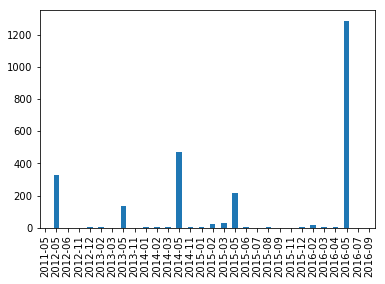
\includegraphics[width=\columnwidth]{figures/freq_month_eurovision.png}
  \vspace{-5mm}
  \caption{For the top months, plot the number of tweets with  \texttt{\#eurovision}}
  \label{fig:freq_month_eurovision}
\end{figure}

With frequency visualisation, we can visualize spikes in the number of tweets. The method \texttt{plot\_frequency\_tags(...)} computes for a given hashtag the numbers of tweets per frequency that contain this hashtag. Here we can chose frequency as either day, month or year. Then it takes the \texttt{n} most tweeted dates and displays them in chronological order with a bar plot. We only take the \texttt{n} most tweeted dates because it provides the most compact visualisation. Note however that these plot are not homogenous in time. 

Now, let us look a the frequency plot \ref{fig:freq_month_eurovision} for \texttt{\#eurovision} .
We can very clearly see an increase in the number of tweet during the month of may of each years. Since eurovision takes place in may, it is obvious that people will more likely talk about it during it's happening. We will be using this knowledge to develop an algorithm to detect those sudden spikes.

\subsection{Visualizing event localisation}

\begin{figure}[htbp]
  \vspace*{-1mm}
  \centering
  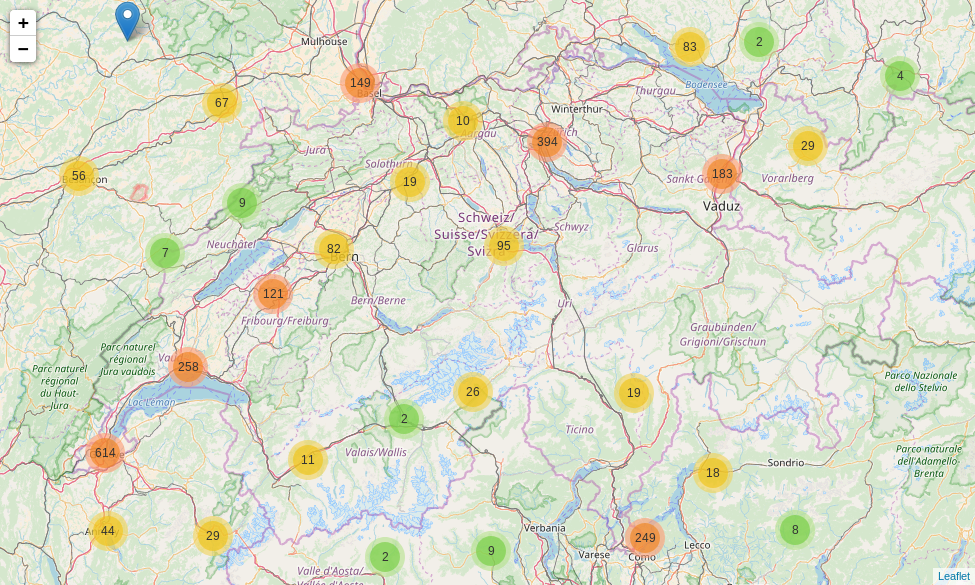
\includegraphics[width=\columnwidth]{figures/map_eurovision.png}
  \vspace{-5mm}
  \caption{Map with every tweet for \texttt{\#eurovision}}
  \label{fig:map_eurovision}
\end{figure}

\begin{figure}[htbp]
  \vspace*{-1mm}
  \centering
  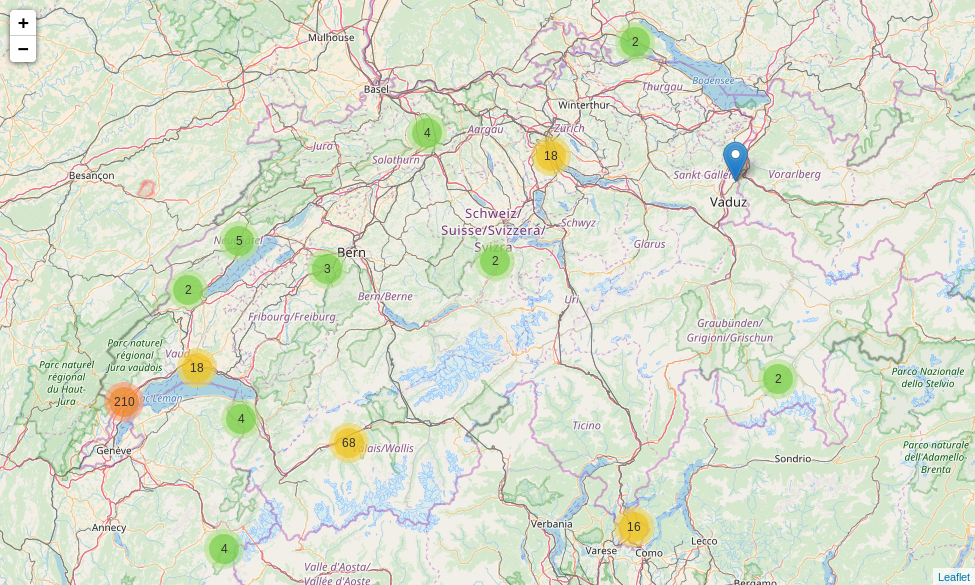
\includegraphics[width=\columnwidth]{figures/map_paleo.png}
  \vspace{-5mm}
  \caption{Map with every tweet for \texttt{\#paleo}}
  \label{fig:map_paleo}
\end{figure}

The map are displayed in order to get an intuition on the geographic repartitions of tweets. The map are created using folium. We use a MarkerCluster to group every tweet close in space. Other than that, it is a pretty straightforward folium map. Now, look at the first map\ref{fig:map_eurovision}. We see that the distribution is regrouped in the cities but overall it is quite uniform if we consider the population density. On the other side, in the second map \ref{fig:map_paleo}, we see that most of the tweets are located in Nyon, which is indeed where this music festival takes place. The logic here people close to the actual event are much more likely to talk about it. Whereas international event are known in switzerland as a whole. Hence a local events lead to tweet localisation around the position of the event and international events have a spread tweet geographic distribution. We will use this knowledge to find the type of an event.


\section{Event detection}

In this part of the project we focus on automatic event detection.

\subsection{Filtering out irrelevant hashtags}

In the data manipulation, we constructed a dictionary containing each hashtag and their respective number of post and unique authors.
Since hashtags that do not have enough posts and that are posted by only a few users are not likely to be considered events by our detection algorithm. We will be filtering out every hashtag that have less than \texttt{100} overal posts and less than \texttt{50} total authors. 

\subsection{Main Challenges}
There were two main challenges we faced when trying to come up with an accurate event detection algorithm. 

The first one is that our dataset spans almost 7 years (from early 2010 to late 2016) and thus the frequency of tweets is obviously much higher at the end of our dataset than at the beginning, as shown in Figure \ref{fig:tweets_year}. Therefore, we had to compare the popularity of a hashtag at a certain date to some kind of baseline, so that our results can adapt to the increasing number of tweets.

\begin{figure}[htbp]
  \vspace*{-1mm}
  \centering
  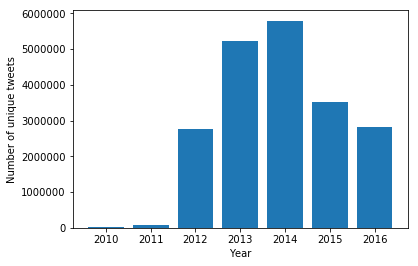
\includegraphics[width=\columnwidth]{figures/tweets_years.png}
  \vspace{-5mm}
  \caption{Number of tweets per years in our dataset. Note that the years 2010 and 2016 are not included in full in the dataset.}
  \label{fig:tweets_year}
\end{figure}

The second challenge is that there are multiple types of events, and they can have very different characteristics. For example, for an event that is scheduled to happen at a certain date, the number of tweets about it gradually increases up to that date. Whereas for a sudden unpredictable event, nobody talks about it and then a big peak happens at the time of the event. Moreover, some events might last multiple days or even weeks, as opposed to one day. Therefore this makes it harder to find an algorithm that detects well all types of events.

\begin{figure}[htbp]
  \vspace*{-1mm}
  \centering
  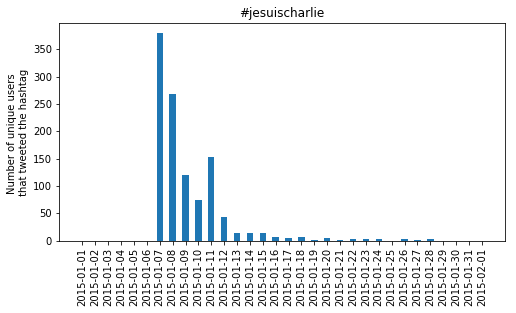
\includegraphics[width=\columnwidth]{figures/freq_event_type1.png}
  \vspace{-5mm}
  \caption{Example of an unpredictable event}
  \label{fig:unpredictable_event}
\end{figure}

\begin{figure}[htbp]
  \vspace*{-1mm}
  \centering
  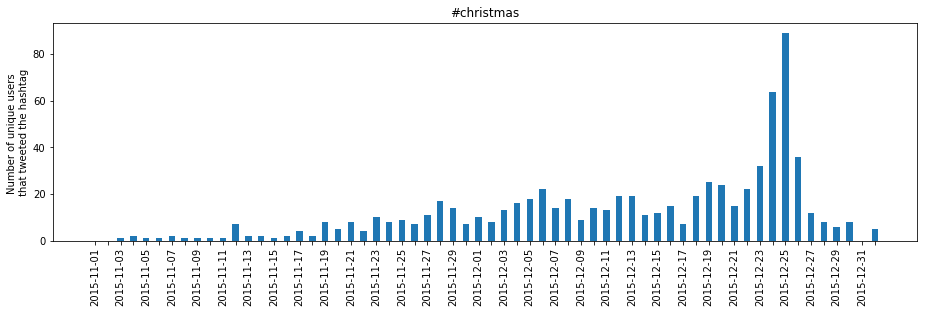
\includegraphics[width=\columnwidth]{figures/freq_event_type2.png}
  \vspace{-5mm}
  \caption{Example of a predictable event}
  \label{fig:predictable_event}
\end{figure}

\subsection{Event Detection Algorithm}
\subsubsection{Algorithm setup}
First of all, we decided to use as a metric of hashtag popularity the number of unique users that tweeted that hashtag. We think this is more relevant than using the total number of tweets, because it prevents us from detecting events based on tweets that were posted by a few users only (e.g. twitter bots or extremely active users). For simplicity, we also decided to detect only the day when an event happens, and not the time, as it would be more complicated. Thus, our algorithm needs as input only the number of unique authors that tweeted a given hashtag, for each day spanned by our dataset, and for each hashtag.

\subsubsection{Algorithm description}
The main idea of our event detection algorithm is to compute what we will call an \textit{event score}, for each day spanned by our dataset and for each hashtag. Then, we apply a threshold on that event score to get dates that are detected as an event.
The event score is obtained by dividing some absolute measure of popularity, by a baseline. That baseline is obtained by computing an average of the number of unique users that tweeted the hashtag over some odd number of days $N$ around the day for which we compute the event score. Dividing by this baseline solves the first problem we talked about. The absolute measure of popularity is obtained by a local weighted average over some odd number of days $M$ around the day for which we compute the event score, where $M << N$.
More specifically, if the number of unique users that tweeted a hashtag at a certain day $d$ is given by $U_d$, and that the kernel for the local weighted average is given by 

$$ K = \big[ w_{ \floor{ -\frac{M}{2} } }  \dots w_{0}  \dots  w_{ \floor{ \frac{M}{2} } } \big] $$

then, the event score at day $d$ is obtained by :

$$ 
event\_score(d) =  \frac {\sum_{i=-\frac{M}{2}}^{\frac{M}{2}} w_i * U_{d + i} }
				    {\frac{1}{N} \sum_{j=-\frac{N}{2}}^{\frac{N}{2}}  U_{d + j} }
$$

The kernel for the weighted local average should be some kind of gaussian, so that the maximum weight is for day $d$. The aim of this local weighted average is to better detect anticipated events, or events lasting a few days. This was implemented to address the second challenge mentioned earlier. 

\subsubsection{Grouping events in time}
After running the algorithm described above, we have a list of hashtags, and the corresponding days where the event score was above the threshold. What we do next is group this list of days for each hashtag so that the dates that are very close are represented as one event over multiple days. More specifically, we grouped two dates together if they were at most 2 days apart.

\subsubsection{Parameters used}
To detect events on the Swiss tweets dataset, we used the following parameters:

$$N = 35 $$
$$M = 3$$
$$K = \big[ 0.1\ \ 0.8\ \ 0.1 \big]$$
$$threshold = 4$$

\section{Event Localization}
Now that we have a list of events, we want to determine the location of an event based on the latitude/longitude data from the tweets that caused this event to be detected. To do so, we chose to compute the median of the latitude and longitude of the tweets. 

But for event that are not necessarily physically happening at some place or that are just trends, a location might not be relevant. Thus in order to determine if the event location is any good, we also compute the mean standard deviation between the computed event location and the location of the tweets. Then we decide that an event is local if the mean standard deviation is below a threshold. If it is not, the event location computed is most likely not relevant and thus we drop it.

\section{Results}
Here are some statistics to quantify our results:

\begin{itemize}
  \item Out of 6197 different hashtag on which we run the event detection algorithm, we found events for 2108 of them.
  \item By grouping by similar dates, we then found 7028 different events.
  \item Out of these 7028 events, we found a relevant location for 440 of them.
\end{itemize}

\subsection{Event Detection}
We correctly detected the events we took as example previously, mainly \#jesuischarlie and \#christmas, as we can see in Figure \ref{fig:christmas} and \ref{fig:jesuischarlie}. Actually, for \#christmas, we detected events on the 24th and 25th of every year between 2012-2015, which is quite good (Note that december 2016 was not included in our dataset).

And more generally, by looking at the events we detected, we can recognise a lot of them as real events. We indeed detect events such as music festivals, conferences, art exhibitions, sporting events, holidays, and much more.
\begin{figure}[htbp]
  \vspace*{-1mm}
  \centering
  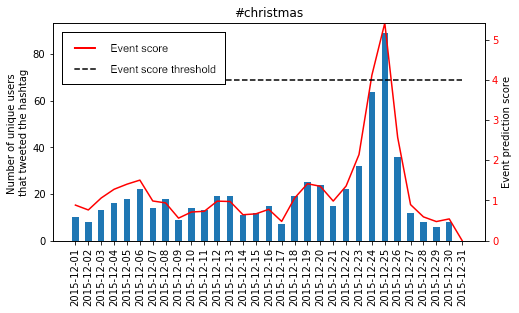
\includegraphics[width=\columnwidth]{figures/christmas_result.png}
  \vspace{-5mm}
  \caption{Computed event score (in red) for the event \#chrismas}
  \label{fig:christmas}
\end{figure}

\begin{figure}[htbp]
  \vspace*{-1mm}
  \centering
  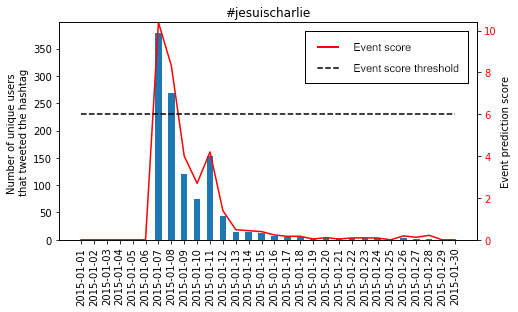
\includegraphics[width=\columnwidth]{figures/jesuischarlie_result.png}
  \vspace{-5mm}
  \caption{Computed event score (in red) for the event \#jesuischarlie}
  \label{fig:jesuischarlie}
\end{figure}

\subsection{Event Localization}
A map containing all 440 events for which a location was found is shown in Figure \ref{fig:events_map}. Unsurprisingly, we can see that most of the events happen in cities, they are especially numerous in Geneva and Z\"urich.

\begin{figure}[htbp]
  \vspace*{-1mm}
  \centering
  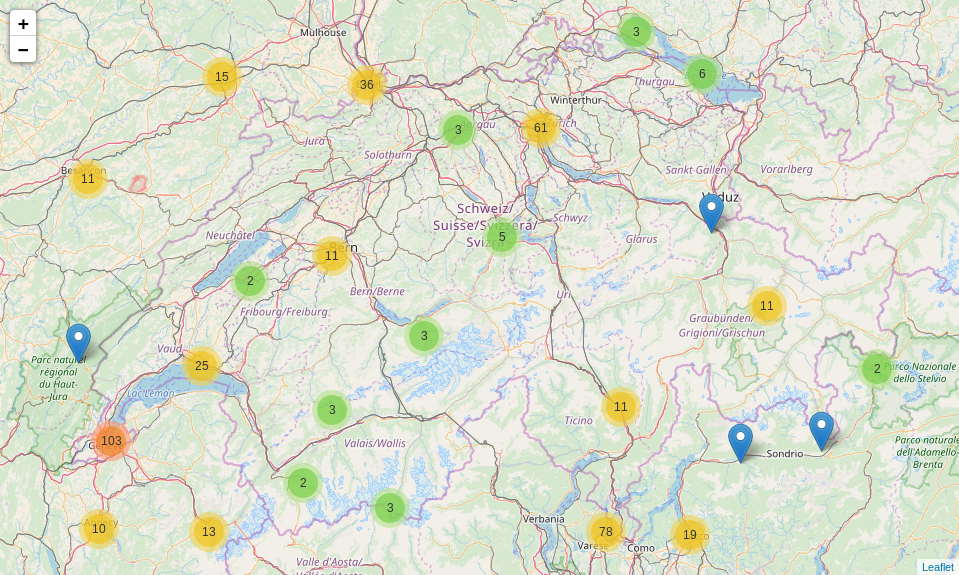
\includegraphics[width=\columnwidth]{figures/local_event_map.png}
  \vspace{-5mm}
  \caption{Map of all localized events}
  \label{fig:events_map}
\end{figure}

\section{Conclusion}



\end{document}
